
\chapter{Vérification et validation de programmes}
\label{sec:existant}

\chapterintro

Le domaine de la vérification et de la validation regroupe un ensemble de
techniques du cycle de développement des logiciels qui ont pour objectif de
s'assurer de leur correction et de leur sûreté. Ces deux notions sont apparues
dans les années soixante-dix avec les travaux de \bsc{Dijkstra}
\cite{Dijkstra/75}, \bsc{Floyd} \cite{Floyd/63} et \bsc{Hoare} \cite{Hoare/69}.

La correction d'un logiciel représente le respect de l'implémentation par
rapport aux spécifications. La sûreté d'un logiciel est liée à son absence
d'erreurs à l'exécution.


\section{Model-checking}
\label{sec:model-checking}

Le model-checking \cite{Clarke/86} permet de vérifier algorithmiquement si
un modèle donné (le système ou une abstraction de ce système) satisfait une
spécification, formulée en termes de logique temporelle \cite{Clarke/82}.
Un modèle est un ensemble d'états, de propriétés que vérifie chaque état, et de
transitions entre ces états qui décrivent l'évolution du système.

Le model-checking couvre l'ensemble des états du système et des transitions afin
d'analyser toutes les exécutions possibles du système. Sur de grands systèmes,
cette méthode est pénalisée par l'explosion combinatoire du nombre des états (et
la complexité en temps ou en espace qui en résulte). Il est néanmoins possible
de modéliser des algorithmes asynchrones répartis et des automates non
déterministes, comme le fait notamment l'outil \spin \cite{\citespin}.

La plateforme \framac intègre \textsc{Aoraï}, un greffon
permettant d'annoter automatiquement le code source d'un programme C d'après
une formule de logique temporelle linéaire, de sorte que les annotations sont
vérifiées si le programme repecte la formule.




\section{Analyse statique}
\label{sec:AS}


\subsection{Langages de spécification}
\label{sec:speclang}


\subsubsection*{Java Modeling Language (\jml)}
\label{sec:jml}

TODO


\subsubsection*{ANSI/ISO C Specification Language (\acsl)}
\label{sec:acsl}

TODO

L'analyse statique \cite{Nielson/99} examine le code source du programme
sans l'exécuter. Elle raisonne sur tous les comportements qui pourraient
survenir lors de l'exécution et permet donc de déduire des propriétés devant
être vérifiées pour toutes ces exécutions, dans le but de prouver la correction
du programme.

En revanche, la vérification de programme étant en général indécidable
\cite{Landi/92}, il est souvent nécessaire d'utiliser des
sur-approximations, ce qui implique que les résultats peuvent être moins précis
que ce que l'on souhaite mais ils sont garantis pour toutes les exécutions.
Ainsi, on peut établir des propriétés de sûreté ({\em safety}), où l’on cherche
des invariants sur les valeurs des variables du programme (une plage de valeurs
par exemple), afin d'exclure certains risques d'erreurs à l'exécution.

Parmi les méthodes statiques sont distinguées : l'interprétation abstraite
(section~\ref{sec:interpretation-abstraite}), l'abstraction à base de
prédicats (section~\ref{sec:abstraction-predicats}) et la preuve de programmes
(section~\ref{sec:preuve}).


\subsection{Interprétation abstraite}
\label{sec:interpretation-abstraite}

L'interprétation abstraite \cite{Cousot/92} s'appuie sur les
théories du point-fixe et des domaines pour introduire des sur-approximations
des comportements d'un programme. Elle consiste à abstraire les domaines des
variables par des domaines finis et beaucoup plus petits. Par exemple, le
domaine des entiers pourrait être abstrait par un domaine de trois valeurs :
$(-, 0, +)$. Appliquée à l’analyse de valeurs, elle consiste à calculer à
chaque ligne du code une sur-approximation de l’ensemble des valeurs prises par
chaque variable en cette ligne lors de toutes les exécutions du programme,
permettant ainsi de détecter certaines erreurs comme les divisions par zéro ou
les accès en dehors des bornes des tableaux.

Pour contourner le problème d’indécidabilité, la théorie de l’interprétation
abstraite construit une méthode qui, à la même question, répondra ``oui'',
``non'' ou ``peut-être''. Si la méthode répond ``peut-être'', c’est qu’on n’a pu
prouver ni l’un ni l’autre des deux premiers cas. C’est ce qu’on appelle une
alarme : il est possible qu’une des exécutions du programme produise une erreur
donnée, mais nous n’avons été capable ni de le confirmer ni de l’infirmer.
L’erreur signalée par une alarme peut ne jamais apparaître à l’exécution, dans
ce cas on l’appelle fausse alarme. On ne calcule donc pas la propriété exacte
mais une abstraction de cette propriété, en imposant la contrainte de sûreté
suivante : ``la propriété abstraite calculée ne doit oublier aucune exécution
concrète''. L'abstraction est effectuée à base de prédicats atomiques
définissant des abstractions des domaines des variables.

\polyspace \cite{\citepolyspace} a été le premier outil commercial
utilisant l'interprétation abstraite pour détecter les erreurs à l'exécution
dans les programmes en C, C++ et Ada mais signale beaucoup de fausses alarmes.
L'ENS a développé \astree \cite{\citeastree}, spécifique au langage C et aux
logiciels critiques. \fluctuat \cite{\citefluctuat},
qui mesure précisément les approximations faites à l'exécution d'un programme C.
\framac intègre un greffon d'interprétation abstraite : \Value
\cite{\citevalue}.



\subsection{Abstraction à base de prédicats}
\label{sec:abstraction-predicats}

L'abstraction à base de prédicats \cite{Schiller/OOPSLA12} est une
technique permettant de générer automatiquement des abstractions de systèmes au
nombre d'états infini. Pour un programme $P$ au nombre d'états infini, un
ensemble fini de prédicats $E = \{f_1, ..., f_n\}$ est défini, ces prédicats
sont des expressions booléennes sur les variables de $P$ et les constantes du
langage.

Chaque état concret de $P$ est mis en correspondance avec un état abstrait de
l'abstraction de $P$, après évaluation par les prédicats de $E$. Un état
abstrait est un $n$-upplet de valeurs booléennes correspondant à la
satisfaisabilité des $n$ prédicats (au moyen d'un solveur SMT).

Par exemple, si 3 prédicats $f_1, f_2, f_3$ sont définis et que la
satisfaisabilité de ces prédicats à l'état concret $e$ est évaluée
respectivement à $false, true, true$, alors dans l'abstraction générée, l'état
$e$ correspond à l'état abstrait $(\lnot f_1, f_2, f_3)$.

L'abstraction générée comporte un nombre fini d'états (au plus $2^n$) car il n'y
a qu'un nombre fini de prédicats, le model-checking peut donc être appliqué à
cette abstraction. Si une propriété de sûreté est vérifiée dans l'abstraction,
elle l'est également dans le système concret.

Cette technique est notamment utilisée par \slam \cite{\citeslam}.


\subsection{Preuve de programmes}
\label{sec:preuve}

La preuve de programmes utilise des fondements mathématiques et logiques
\cite{Hoare/69} pour prouver des propriétés de programmes. Tout d'abord, le
système
est décrit par un ensemble d'axiomes et de règles d'inférence. Puis, le calcul
de la plus faible précondition \cite{Dijkstra/75} est utilisé pour générer des
formules appelées obligations de preuve, qui sont finalement soumises à un
prouveur de théorèmes, qui applique différentes techniques de résolution.

Contrairement au model-checking, la preuve a l'avantage d'être
indépendante de la taille de l'espace des états, et peut donc s'appliquer sur
des systèmes de grande taille. En contre-partie, cette technique requiert une
expertise de l'utilisateur pour adapter le programme à la preuve (en l'annotant
par exemple) et guider le prouveur si nécessaire.

Il existe des prouveurs automatiques tels que \simplify \cite{\citesimplify},
\ergo \cite{\citeergo} et \zthree \cite{\citezthree}; et des
prouveurs interactifs, où la preuve est guidée par l'utilisateur, tels que
\coq \cite{\citecoq}, \isabelle \cite{\citeisabelle}, et \hol \cite{\citehol}.
Certains de ces prouveurs ou assistants de preuve sont intégrés à
d'autres outils tels \boogie \cite{\citeboogie} ou \escjava \cite{\citeescjava}.
\framac intègre le greffon de preuve, \Wp \cite{\citewp} qui traite des
programmes dont le code contient des annotations \acsl \cite{\citeacsl}.


\section{Analyse dynamique}
\label{sec:AD}


L’analyse dynamique est basée sur des techniques d’exécution du programme, de
simulation \cite{Whitner/WSC89} d’un modèle ou d'exécution symbolique
\cite{Clarke/76}, regroupées sous le terme générique ``test''.

Les tests peuvent s’appliquer tout au long du cycle de développement d’un
logiciel. Les tests unitaires vérifient le bon fonctionnement des différentes
entités d’un système, indépendamment les unes des autres. Les tests
d'intégration vérifient la bonne communication entre ces entités. Les tests de
validation s'assurent que les fonctionnalités correspondent au besoin de
l’utilisateur final. Enfin, les tests de non-régression vérifient que l'ajout de
nouvelles fonctionnalités ne détériore pas les anciennes fonctionnalités.

En général, les techniques de test ne sont pas exhaustives et n'explorent qu'un
sous-ensemble des chemins d'exécutions du programme, en conséquence, l’absence
d’échecs lors du passage des tests n’est pas une garantie de bon fonctionnement
du système. Néanmoins, selon les critères utilisés pour la génération des
tests, et selon la couverture des chemins d'exécution fournie par les tests, un
système ainsi validé peut acquérir un certain niveau de confiance.

Les méthodes de test peuvent être classées en trois catégories : le test
aléatoire, le test structurel (section~\ref{sec:test-structurel}) et le test
fonctionnel (section~\ref{sec:test-fonctionnel}). Comme son nom l'indique, le
test aléatoire consiste à générer des valeurs d'entrée du programme au hasard et
ne sera pas détaillé dans cette thèse.


\subsection{Langages de spécification exécutables}
\label{sec:execspeclang}


\subsubsection*{\textsc{Executable-acsl} (\eacsl)}

\eacsl est un sous-ensemble ``exécutable'' du langage \acsl
implémenté dans \framac. Contrairement à \acsl, chaque
spécification \eacsl est exécutable : elle peut être évaluée à
l'exécution.


\subsection{Exécution symbolique pour le test structurel}
\label{sec:exec-sym}



\subsubsection*{Exécution symbolique augmentée}



\subsection{Test structurel}
\label{sec:test-structurel}

Le test structurel, ou test ``boîte blanche'', est une technique de test qui
fonde la détermination des différents cas de test sur une analyse de la
structure du code source du programme étudié. On distingue deux types de tests
structurels : le test orienté flot de contrôle et le test orienté flot de
données.

Le test orienté flot de données cherche à couvrir certaines relations entre la
définition d’une variable et son utilisation, par exemple, on peut souhaiter
couvrir toutes les lectures d'une variable suivant une écriture.

Le test orienté flot de contrôle s’intéresse quant à lui à la structure du
programme : l'ordre dans lequel les instructions sont exécutées. Il se base sur
le graphe de flot de contrôle du programme : un graphe connexe orienté avec un
unique n\oe{}ud d’entrée et un unique n\oe{}ud de sortie, dont les n\oe{}uds
sont les blocs de base du programme et les arcs représentent les branchements
(conditions). Une couverture structurelle de ce graphe est recherchée, selon un
critère qui peut être par exemple ``toutes les instructions'',
``toutes les branches'' (toutes les décisions), ``tous les chemins'' ou
``tous les $k$-chemins''.

L’exécution symbolique dynamique, ou exécution ``concolique'', associe
l’exécution concrète du programme et l’exécution symbolique afin d’explorer les
chemins du programme. L’exécution concrète sert à confirmer que le chemin
parcouru est bien celui pour lequel le cas de test exécuté a été généré.

Plusieurs outils se basent sur l'exécution concolique pour explorer un programme
sous test, dont \smart \cite{\citesmart}, \pex \cite{\citepex},
\sage \cite{\citesage}, \cute \cite{\citecute}, \klee \cite{\citeklee},
\exe \cite{\citeexe}, \pathcrawler \cite{\citepathcrawler}. Ces outils
utilisent des solveurs de contraintes pour générer des cas de test permettant
d'aboutir à une couverture souhaitée des exécutions du programme par les tests.


\subsubsection*{\pathcrawler}

\pathcrawler \cite{\citepathcrawler} est un outil de génération de tests
structurels pour les programmes C, accessible sous la forme d'un service web :
\textsc{PathCrawler Online} \cite{\citepconline}.

Étant donné un programme C sous test $p$ et une pré-condition sur ses entrées,
il génère des cas de test respectant un critère de couverture de test. Le
critère \emph{tous les chemins} impose une couverture de tous les chemins
faisables de $p$. L'exploration exhaustive de tous les chemins étant en pratique
irréalisable sur des programmes réels, le critère \emph{tous les k-chemins} a
été défini, il limite l'exploration aux chemins qui ont au plus $k$ itérations
consécutives de chaque boucle.

\pathcrawler commence par construire une version instrumentée de $p$
permettant de tracer l'exécution de chaque cas de test, puis il génère les
contraintes représentant la sémantique de chaque instruction de $p$. La
prochaine étape est la génération et la résolution de contraintes pour produire
les cas de test pour un ensemble de chemins $\Pi$ satisfaisant le critère de
couverture. La résolution de contraintes s'effectue à l'aide
d'\eclipse \prolog \cite{\citeeclipse}, un environnement de programmation en
logique par contraintes basé sur \prolog.

Étant donné un préfixe de chemin $\pi$, c'est-à-dire un chemin partiel de $p$,
l'idée est de résoudre les contraintes correspondant à l'exécution symbolique
de $p$ en suivant le chemin $\pi$.
 
La méthode de génération de test est composée des étapes suivantes :

\begin{itemize}
\item[$(\mathcal{G}_1)$]
Création d'une variable logique pour chaque entrée.
Prise en compte des contraintes de la pré-condition.
Le préfixe de chemin initial $\pi$ est vide.
Aller à $(\mathcal{G}_2)$.

\item[$(\mathcal{G}_2)$]
Exécuter symboliquement le chemin $\pi$ : ajout des contraintes et
mise à jour de la mémoire en fonction des instructions de $\pi$.
Si certaines contraintes sont insatisfiables, aller à $(\mathcal{G}_5)$.
Sinon, aller à $(\mathcal{G}_3)$.

\item[$(\mathcal{G}_3)$]
Appeler le solveur de contraintes pour générer un cas de test $t$ satisfaisant
les contraintes du chemin courant. Si les contraintes sont insatisfiables, aller
à $(\mathcal{G}_5)$.
Sinon, aller à $(\mathcal{G}_4)$.

\item[$(\mathcal{G}_4)$]
Exécuter le programme avec trace sur le cas de test $t$ généré pour obtenir
le chemin d'exécution, qui doit commencer par $\pi$.
Aller à $(\mathcal{G}_5)$.

\item[$(\mathcal{G}_5)$]
Calculer le prochain chemin partiel $\pi$ à couvrir. Un parcours en profondeur
détermine la dernière décision $d$ pour laquelle il reste une branche à
explorer. S'il n'existe pas une telle décision, l'algorithme s'arrête. Sinon,
$\pi$ est recalculé et contient maintenant le chemin partiel précédent dans
lequel les contraintes correspondant à $d$ ont été niées, et retour à l'étape
$(\mathcal{G}_2)$. Cela nous assure que tous les chemins faisables sont couverts
(en considérant que le solveur de contraintes peut trouver une solution dans un
temps raisonnable) et que seulement le plus court des préfixes infaisables de
chaque chemin infaisable est exploré.
\end{itemize}



\subsection{Test fonctionnel}
\label{sec:test-fonctionnel}

Le test fonctionnel, ou test ``boîte noire'', génère des jeux de test en
fonction du comportement attendu du programme : un cas de test sera choisi pour
chaque comportement particulier. Le test fonctionnel est utilisé pour vérifier
la conformité des réactions du logiciel avec les attentes de l'utilisateur, sans
connaissance du code source. Il existe de nombreuses techniques qui se
différencient par la manière de choisir les données de test, parmi lesquelles :

\begin{description}
\item[le test de partition] \hfill \\
les valeurs d’entrées du logiciel sont regroupées en classes d’équivalence, sur
lesquelles le logiciel doit avoir le même comportement ({\em domain splitting}),
une seule valeur aléatoire est choisie dans chaque classe de la partition;
\item[le test aux limites] \hfill \\
les données de test sont choisies aux bornes des domaines de définition des
variables.
\end{description}

\gatel \cite{\citegatel} est un générateur de
tests fonctionnels qui se base sur une représentation symbolique des états du
système : le programme, les invariants et les contraintes décrivant l'objectif
de test sont exprimés dans le langage \lustre \cite{\citelustre}. Cet outil
offre la possibilité de réaliser des partitions de domaines.



\subsection{Monitoring}
\label{sec:monitoring}


TODO


\section{Combinaisons statique/dynamique}
\label{sec:combinaison}

Les méthodes statiques et les méthodes dynamiques ont des avantages et des
inconvénients complémentaires : l'analyse statique étant complète mais
imprécise, l'analyse dynamique étant précise mais incomplète. L’idée de les
combiner pour associer leurs avantages et combattre leurs inconvénients
\cite{Ernst/WODA03} est une voie de recherche active et fructueuse dans le
domaine de la vérification de programmes.


\subsubsection*{\textsc{Static ANalysis and TEst}}

La méthode \sante \cite{Chebaro/11, \citesante}, mise en \oe{}uvre au sein de
\framac, combine l'interprétation abstraite, le {\em slicing} et la
génération de tests structurels avec \pathcrawler. L’analyse statique
signale les instructions risquant de provoquer des erreurs à l’exécution par des
alarmes, dont certaines peuvent être de fausses alarmes, puis l’analyse
dynamique génère des tests confirmant ou infirmant ces alarmes. Sur des
programmes de grande taille, l'analyse dynamique peut manquer de temps pour
classer toutes ces alarmes (à cause de l'explosion combinatoire des exécutions
possibles). Le {\em slicing} est utilisé pour réduire la taille des programmes
testés et donc le temps nécessaire à leur analyse.

Le fonctionnement général de la méthode est illustré par la
Fig.~\ref{figSlicing} ~\textbf{a}. Cette méthode utilise l'analyse de valeurs
(interprétation abstraite) afin de sélectionner les instructions pour lesquelles
le risque d'une erreur à l'exécution n'est pas écarté (nous les appellerons
``alarmes'' par la suite), par exemple une division par zéro ou un accès
invalide à la mémoire.

Ces alarmes vont être validées par des tests. Nous utilisons
\pathcrawler \cite{\citepathcrawler}, un outil de génération de tests
structurels, pour tenter de mettre en évidence un cas de test pour lequel le
chemin d'exécution passe par cette alarme, et provoque une erreur.

Pour diminuer le coût de la génération de tests, nous simplifions
syntaxiquement les programmes qui lui seront soumis pour ne garder que les
instructions dont dépend l'alarme considérée, on appelle cette opération
{\em slicing} \cite{Korel/88}. Nous obtenons ainsi des programmes plus simples,
tels que si une alarme est présente dans le programme d'origine, elle l'est
également dans les programmes simplifiés si le {\em slicing} a été paramétré
pour conserver les instructions dont dépend cette alarme. Et si elle provoque
une erreur dans le programme d'origine, alors il en sera de même dans les
programmes simplifiés, avec les mêmes entrées. L'utilisation du {\em slicing}
peut être paramétrée par différentes options, qui seront détaillées plus bas.

La première phase de la méthode (l'interprétation abstraite) peut donc assurer
que certaines instructions ne provoqueront pas d'erreur à l'exécution, tandis
que la seconde phase permet de confirmer que certaines alarmes produisent
effectivement une erreur à l'exécution. Et la mise en commun des résultats des
deux phases permet de classifier davantage d'alarmes dans l'une ou l'autre de
ces deux catégories que chacune des deux méthodes prise séparément. La preuve de
la correction de cette méthode et le résultat des analyses comparées sont
détaillés dans \cite{Chebaro/11} et \cite{\citesante} et ne seront pas répétés
ici.


\begin{figure}[h]
  \begin{center}
    
    %\hfill{}
    \begin{tabular}{cccc}

      \begin{pspicture}(0,0)(6,6.7)
        \centering

        \rput[tl](0,6.6){\ovalnode{P}{\scriptsize{$\lefteqn{\mbox{Program}\,p}\phantom{Preond p pre}$}}}
        \rput[tr](5.3,6.6){\ovalnode{Context}{\scriptsize{$\lefteqn{\mbox{Precondition}}\phantom{Preond p pre}$}}}

        \rput(2.5,5.5){\rnode{VA}{\psshadowbox[shadowsize=0,fillcolor=red!10,fillstyle=solid]{
              \centering \begin{scriptsize}\begin{tabular}{c}Value Analysis
                  %\\(Frama-C plugin)
        \end{tabular}\end{scriptsize}}}}
        \rput(2.5,4.6){\ovalnode{VA-SL}{\scriptsize{$\lefteqn{\!\!\!\!p,\, A = \alarms(p)}\phantom{aaaaaaaaaaa}$}}}   
        \rput(2.5,3.7){\rnode{SL}{\psshadowbox[shadowsize=0,fillcolor=red!10,fillstyle=solid]{
              \begin{scriptsize}\begin{tabular}{c}$\SliceTest$\end{tabular}\end{scriptsize}}}}
        
        \rput[tr](0.8,4.1){\rnode{SLOP}{\begin{scriptsize}\begin{tabular}{l} Option:
                \textit{none},\\
                \textit{all}, \textit{each}, \\
                \textit{min}, \textit{smart}\end{tabular}\end{scriptsize}}}

        \rput(2.5,2.9){\ovalnode{Diagnostic}{\scriptsize{Diagnostic}}}
        \rput(0.05,6.7){\textbf{a)}}
        
        \ncline[]{->}{P}{VA}
        \ncline[]{->}{Context}{VA}

        \ncline[nodesep=0pt]{->}{VA}{VA-SL}
        \ncline[nodesep=0pt]{->}{VA-SL}{SL}
        \ncline[nodesep=0pt]{->}{SLOP}{SL}
        
        \ncline[]{->}{SL}{Diagnostic}
      \end{pspicture}

     &
      
      \begin{pspicture}(0,0)(3.5,7)
        \centering

        \rput(1.75,6.9){\ovalnode{allInput}{\scriptsize{\raisebox{-0.5mm}[0.9mm][1mm]{$p,\,A$}}}}
        \rput(1.75,4.37){\rnode{SL}{\psshadowbox[shadowsize=0,fillcolor=red!10,fillstyle=solid]{
              \parbox{3.5cm}{\begin{tabular}{c} \\ \\ \\ \\ \\ \\ \\ \end{tabular}}
        }}}
        \rput(1.75,5.7){\rnode{SEL}{\psshadowbox[shadowsize=0,fillcolor=blue!10,fillstyle=solid]{\parbox{3cm}{\centering\scriptsize{Select \textit{all}}}}}}
        \rput(1.75,4.8){\rnode{SLICE}{\psshadowbox[shadowsize=0,fillcolor=blue!10,fillstyle=solid]{\parbox{3cm}{\centering\scriptsize{Slice}}}}}
       
        \rput(1.75,4.0){\ovalnode{allOutput}{\scriptsize{\raisebox{-0.5mm}[0.2mm][1mm]{$p_{A}$}}}}
        \rput(1.95,5.32){\scriptsize{$A$}}

        \rput(1.75,3.1){\rnode{DA}{\psshadowbox[shadowsize=0,fillcolor=blue!10,fillstyle=solid]{\parbox{3cm}{\centering\scriptsize{Dynamic Analysis}}}}}
        \rput(0.05,6.7){\textbf{b)}}
        \rput(1.75,1.8){\ovalnode{Diagnostic}{\scriptsize{\raisebox{-0.5mm}[1mm][1mm]{$Diagnostic$}}}}
        \ncline[nodesep=0pt]{->}{allInput}{SL}
        \ncline[nodesep=0pt]{->}{SEL}{SLICE}
        \ncline[nodesep=0pt]{->}{SLICE}{allOutput}
        \ncline[nodesep=0pt]{->}{allOutput}{DA}
        \ncline[]{->}{DA}{Diagnostic}
      \end{pspicture}
      
      
      & &
      
      %each
      \begin{pspicture}(0,0)(3.5,7)
        \centering
        \rput(1.75,6.9){\ovalnode{allInput}{\scriptsize{\raisebox{-0.5mm}[0.9mm][1mm]{$p,\,A$}}}}
        \rput(1.75,4.37){\rnode{SL}{\psshadowbox[shadowsize=0,fillcolor=red!10,fillstyle=solid]{
              \parbox{3.5cm}{\begin{tabular}{c} \\ \\ \\ \\ \\ \\ \\ \end{tabular}}
        }}}
        \rput(1.75,5.7){\rnode{SEL}{\psshadowbox[shadowsize=0,fillcolor=blue!10,fillstyle=solid]{\parbox{3cm}{\centering\scriptsize{Select \textit{each}}}}}}
        
        \rput(0.6,4.8){\rnode{SLICE1}{\psshadowbox[shadowsize=0,fillcolor=blue!10,fillstyle=solid]{\parbox{0.8cm}{\centering\scriptsize{Slice}}}}}

        \rput(2.9,4.8){\rnode{SLICEn}{\psshadowbox[shadowsize=0,fillcolor=blue!10,fillstyle=solid]{\parbox{0.8cm}{\centering \scriptsize{Slice}}}}}
        
        \rput(0.6,4.0){\ovalnode{p1}{\scriptsize{\raisebox{-0.5mm}[0.2mm][1mm]{$p_{a_1}$}}}}
        \rput(2.9,4.0){\ovalnode{pn}{\scriptsize{\raisebox{-0.5mm}[0.2mm][1mm]{$p_{a_n}$}}}}
        
        \rput(1,5.3){\scriptsize{$\{a_1\}$}}
        \rput(3.3,5.3){\scriptsize{$\{a_n\}$}}
        \rput(1.8,4.8){. . .}

        \rput(1.75,3.1){\rnode{DA}{\psshadowbox[shadowsize=0,fillcolor=blue!10,fillstyle=solid]{\parbox{3cm}{\centering\scriptsize{Dynamic Analysis}}}}}
        \rput(0.05,6.7){\textbf{c)}}
        \rput(1.75,1.8){\ovalnode{Diagnostic}{\scriptsize{\raisebox{-0.5mm}[1mm][1mm]{$Diagnostic$}}}}

        \ncline[nodesep=0pt]{->}{allInput}{SL}



        \ncangle[angleA=-90,angleB=90,offsetA=-1.15]{->}{SEL}{SLICE1}
        \ncangle[angleA=-90,angleB=90,offsetA=1.15,offsetB=0]{->}{SEL}{SLICEn}
        \ncline[nodesep=0pt]{->}{SLICE1}{p1}    
        \ncline[nodesep=0pt]{->}{SLICEn}{pn}    
%        \ncangle[angleA=-90,angleB=90]{->}{SLICE1}{p1}
%        \ncangle[angleA=-90,angleB=90]{->}{SLICEn}{pn}
        \ncangle[angleA=-90,angleB=90,offsetB=-1.15]{->}{p1}{DA}
        \ncangle[angleA=-90,angleB=90,offsetB=1.15]{->}{pn}{DA}
        \ncline[]{->}{DA}{Diagnostic}
      \end{pspicture}
    
    \end{tabular}
\vspace{-14mm}
\caption{\textbf{a)} General overview, Basic $\SliceTest$  options:
\textbf{b)} \textit{all},  \textbf{c)} \textit{each}} 
\label{figSlicing}\vspace{-5mm}
\end{center}
\end{figure}







L'option {\em none} signifie l'absence de {\em slicing} : le programme n'est pas
simplifié et est soumis en l'état à \pathcrawler.

L'option {\em all} (Fig.~\ref{figSlicing} ~\textbf{b}) génère un seul programme
simplifié contenant toutes les alarmes signalées par l'analyse de valeur. Cette
option ne tire pas profit du fait que certaines alarmes peuvent être
indépendantes (et peuvent donc être soumises séparément), la complexité du
programme soumis à \pathcrawler peut l'empêcher de générer des cas de
test pour toutes les alarmes dans le temps qui lui est imparti.

L'option {\em each} (Fig.~\ref{figSlicing} ~\textbf{c}) tente de corriger ce
défaut, elle génère un programme simplifié par alarme et invoque
\pathcrawler autant de fois. Ainsi, les alarmes les plus simples ne sont
pas pénalisées par les plus complexes. Néanmoins, en cas de dépendances
mutuelles entre alarmes, plusieurs programmes identiques seront soumis à
\pathcrawler, ce qui est une perte de temps.

\begin{figure}[h]
\begin{center}
  \mbox{}\hspace{3mm}
	\begin{tabular}{cc}
      %min
      \begin{pspicture}(0,0)(3,12)
        \centering
        \rput(1,11.6){\ovalnode{allInput}{\centering  \scriptsize{\raisebox{-0.5mm}[0.9mm][1mm]{$p,\,A$}}}}

        \rput(1,10.8){\rnode{DEPS}{\psshadowbox[shadowsize=0,fillcolor=blue!10,fillstyle=solid]{
              \parbox{3cm}{\centering \scriptsize{Dependency Analysis}}}}}
        \rput(1,9.9){\ovalnode{DEPS-SL}{\centering  \scriptsize{\raisebox{-1mm}[0.2mm][1mm]{$p,\,A,\,\dep$}}}}

        \rput(1,7.7){\rnode{SL}{\psshadowbox[shadowsize=0,fillcolor=red!10,fillstyle=solid]{
              \parbox{2.9cm}{\begin{tabular}{c}\\ \\ \\ \\ \\ \\ \\ \end{tabular}}
        }}}
       
        \rput(1,9.05){\rnode{SEL}{\psshadowbox[shadowsize=0,fillcolor=blue!10,fillstyle=solid]{\parbox{2.6cm}{\centering\scriptsize{Select \textit{min}}}}}}

        \rput(0.05,8.2){\rnode{SLICE1}{\psshadowbox[shadowsize=0,fillcolor=blue!10,fillstyle=solid]{\parbox{0.7cm}{\centering\scriptsize{Slice}}}}}
        
        \rput(1.95,8.2){\rnode{SLICEn}{\psshadowbox[shadowsize=0,fillcolor=blue!10,fillstyle=solid]{\parbox{0.7cm}{\centering\scriptsize{Slice}}}}}
        
        \rput(0.05,7.3){\ovalnode{p1}{\scriptsize{\raisebox{0mm}[1mm][1mm]{$\,p_{A_1}$}}}}
        \rput(1.95,7.3){\ovalnode{pn}{\scriptsize{\raisebox{0mm}[1mm][1mm]{$\,p_{A_k}$}}}}
        
        
        \rput(0.3,8.65){\scriptsize{$A_1$}}
        \rput(2.2,8.65){\scriptsize{$A_k$}}
        \rput(1,8.3){. . .}

        \rput(1,6.4){\rnode{DA}{\psshadowbox[shadowsize=0,fillcolor=blue!10,fillstyle=solid]{\parbox{2.6cm}{\centering\scriptsize{Dynamic Analysis}}}}}

        \rput(-0.5,11.6){\textbf{a)}}        
        \rput(1,5.4){\ovalnode{Diagnostic}{\scriptsize{\raisebox{-0.5mm}[1mm][1mm]{$Diagnostic$}}}}

        \ncline[nodesep=0pt]{->}{allInput}{DEPS}
        \ncline[nodesep=0pt]{->}{DEPS}{DEPS-SL}

        \ncline[nodesep=0pt]{->}{DEPS-SL}{SL}
        
        \ncangle[angleA=-90,angleB=90,offsetA=-0.95]{->}{SEL}{SLICE1}
        \ncangle[angleA=-90,angleB=90,offsetA=0.95,offsetB=0]{->}{SEL}{SLICEn}
        
        
        \ncangle[angleA=-90,angleB=90]{->}{SLICE1}{p1}
        \ncangle[angleA=-90,angleB=90]{->}{SLICEn}{pn}

        \ncangle[angleA=-90,angleB=90,offsetB=-0.95]{->}{p1}{DA}
        \ncangle[angleA=-90,angleB=90,offsetB=0.95]{->}{pn}{DA}
        \ncline[]{->}{DA}{Diagnostic}
      \end{pspicture}
      
      
      &
      
      \begin{pspicture}(0,0)(4,12)
        \centering
        \rput(1.3,11.6){\ovalnode{allInput}{\centering \scriptsize{\raisebox{-0.5mm}[0.9mm][1mm]{$p,\,A$}}}}
        \rput(2.4,10.35){\begin{scriptsize}$A^0:=A;\,i:=0$\end{scriptsize}}
        
        \rput(1.3,10.8){\rnode{DEPS}{\psshadowbox[shadowsize=0,fillcolor=blue!10,fillstyle=solid]{
              \parbox{3cm}{\centering \scriptsize{Dependency Analysis} }}}}
        \rput(1.3,9.9){\ovalnode{DEPS-SL}{\scriptsize{\raisebox{-1mm}[0.2mm][1mm]{{$p,\,A^i,\,\dep$}}}}}
        
        
        \rput(1.3,7.7){\rnode{SL}{\psshadowbox[shadowsize=0,fillcolor=red!10,fillstyle=solid]{
              \parbox{2.9cm}{\begin{tabular}{c}\\ \\ \\ \\ \\ \\ \\ \end{tabular}}
        }}}
        

        \rput(1.3,9.05){\rnode{SEL}{\psshadowbox[shadowsize=0,fillcolor=blue!10,fillstyle=solid]{\parbox{2.6cm}{\centering\scriptsize{Select \textit{min}}}}}}
        
        \rput(0.3,8.2){\rnode{SLICE1}{
            \psshadowbox[shadowsize=0,fillcolor=blue!10,fillstyle=solid]{
              \parbox{0.7cm}{\centering\scriptsize{Slice}}}}}
        
        \rput(2.2,8.2){\rnode{SLICEn}{
            \psshadowbox[shadowsize=0,fillcolor=blue!10,fillstyle=solid]{
              \parbox{0.7cm}{\centering\scriptsize{Slice}}}}}
        
        \rput(1.3,6.4){\rnode{DA}{\psshadowbox[shadowsize=0,fillcolor=blue!10,fillstyle=solid]{\parbox{2.6cm}{\centering\scriptsize{Dynamic Analysis}}}}}
        
        \rput(0.3,7.3){\ovalnode{p1}{\scriptsize{\raisebox{0.4mm}[1mm][1mm]{$\,\,p_{A^i_{1}}$}}}}
        \rput(2.2,7.3){\ovalnode{pn}{\scriptsize{\raisebox{0.8mm}[1mm][1mm]{$\,p_{A^i_{k_i}}$}}}}
        \rput(3.8,7.7){\ovalnode{Ai}{\scriptsize{\raisebox{-0.4mm}[1mm][0.1mm]{$A^{i+1}$}}}}


        \rput(1.3,5.4){\ovalnode{DIAGi}{\scriptsize{\raisebox{-0.5mm}[1mm][1mm]{$Diagnostic^i$}}}}

        \rput(1.3,4.7){\rnode{FILTER}{\psshadowbox[shadowsize=0,fillcolor=blue!10,fillstyle=solid]{\parbox{3.12cm}{\centering\scriptsize{Refine}}}}}
        
        
        \rput(0.55,8.65){\scriptsize{$A^i_{1}$}}
        \rput(2.5,8.645){\scriptsize{$A^i_{k_i}$}}
        \rput(1.3,8.2){. . .}
        \rput(-0.3,11.6){\textbf{b)}}
        \rput(1.3,3.7){\ovalnode{Diagnostic}{\scriptsize{\raisebox{-0.5mm}[1mm][1mm]{$Diagnostic$}}}}

        \rput(3.8,9.2){\begin{scriptsize}$i:=i+1$\end{scriptsize}}
        \rput(0.6,4.3){\begin{scriptsize}$A^{i+1}=\emptyset$\end{scriptsize}}
        \rput(3.6,4.5){\begin{scriptsize}$A^{i+1}\ne\emptyset$\end{scriptsize}}

        \ncline[nodesep=0pt]{->}{allInput}{DEPS}
        \ncline[nodesep=0pt]{->}{DEPS}{DEPS-SL}

        \ncline[nodesep=0pt]{->}{DEPS-SL}{SL}
        

        \ncangle[angleA=-90,angleB=90,offsetA=-1]{->}{SEL}{SLICE1}
        \ncangle[angleA=-90,angleB=90,offsetA=0.9,offsetB=0]{->}{SEL}{SLICEn}

        \ncline[]{->}{DA}{DIAGi}
        \ncline[]{->}{DIAGi}{FILTER}
        
        
        \ncangle[angleA=-90,angleB=90]{->}{SLICE1}{p1}
        \ncangle[angleA=-90,angleB=90]{->}{SLICEn}{pn}

%        \ncangles[angleA=-90,angleB=-90,arm=0.5,linearc=.15,offsetA=0.5]{->}{FILTER}{Ai}
        \ncangle[angleA=0,angleB=-90, linearc=.15,offsetA=0]{->}{FILTER}{Ai}
        \ncangle[angleA=90,arm=0.6cm, linearc=.15]{->}{Ai}{SEL}
        
        \ncangle[angleA=-90,angleB=90,offsetB=-1]{->}{p1}{DA}
        \ncangle[angleA=-90,angleB=90,offsetB=0.9]{->}{pn}{DA}
%        \ncangle[angleA=-90,angleB=90,offsetA=-0.5]{->}{FILTER}{Diagnostic}
        \ncline[nodesep=0pt]{->}{FILTER}{Diagnostic}
      \end{pspicture}
      
    
    \\
    \\
%    \textbf{a)} Option \textit{min} &
%    \textbf{b)} Option \textit{smart}
    
    \end{tabular}
\vspace{-40mm}
\caption{Advanced $\SliceTest$  options:
\textbf{a)} \textit{min},  \textbf{b)} \textit{smart}} 
\label{figSlicingAdvanced}
\vspace{-5mm}
\end{center}
\end{figure}



L'option {\em min} (Fig.~\ref{figSlicingAdvanced} ~\textbf{a}) tente de corriger
les inconvénients de {\em all} et de {\em each} et propose de générer une
couverture minimale des alarmes par {\em slicing}, de manière à regrouper dans
un même ensemble les alarmes ayant une relation de dépendance \cite{\citesante}.
Considérons par exemple les alarmes $\{a_1; a_2; a_3; a_4; a_5\}$, dont les
dépendances (Fig.~\ref{fig:deps}) sont : $a_2$ dépend de $a_1$; $a_5$ dépend de
$a_4$ qui dépend de $a_3$, qui dépend de $a_1$.
Dans cet exemple, la couverture minimale est constituée des deux ensembles
couvrants $\{a_1; a_2\}$ et $\{a_1; a_3; a_4; a_5\}$.


\begin{figure}
  \centering
  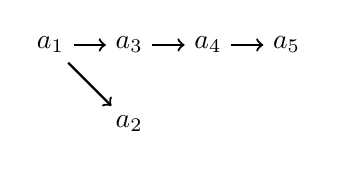
\begin{tikzpicture}
    \node(s) at (0,1) {$a_1$};
    \node(t) at (1,0) {$a_2$};
    \node(q) at (1,1) {$a_3$};
    \node(d) at (2,1) {$a_4$};
    \node(v) at (3,1) {$a_5$};
    \path[->,thick] (s) edge (q);
    \path[->,thick] (q) edge (d);
    \path[->,thick] (d) edge (v);
    \path[->,thick] (s) edge (t);
  \end{tikzpicture}
  \caption{Graphe de dépendances des alarmes}
  \label{fig:deps}
\end{figure}


Chacun de ces ensembles sera utilisé pour générer un programme simplifié ne
contenant que des alarmes ayant une relation de dépendance, évitant ainsi
d'avoir plusieurs programmes identiques en cas de dépendances mutuelles (et
réduisant le nombre d'appels à \pathcrawler).
On remarque que si toutes les alarmes sont dépendantes, on se retrouve dans le
cas de {\em all}, et si elles sont toutes indépendantes, on se retrouve dans le
cas de {\em each}.

Dans le cas où les ensembles couvrants contiennent de nombreuses alarmes,
{\em min} hérite de l'inconvénient de l'option {\em all} : les alarmes les plus
complexes à classifier pénalisent les autres, qui peuvent ne pas être
diagnostiquées dans le temps imparti.

Pour corriger ce défaut, l'option {\em smart} (Fig.~\ref{figSlicingAdvanced}
~\textbf{b}) est définie. Elle consiste à appliquer {\em min} itérativement en
diminuant l'ensemble des alarmes considérées à chaque itération. Les alarmes
supprimées seront des alarmes classifiées ou des alarmes finales.

\begin{definition}[Alarme finale]
Une alarme finale est une alarme dont aucune autre alarme de dépend mais
pouvant avoir des dépendances mutuelles avec d'autres alarmes finales.
Sur notre exemple, $a_2$ et $a_5$ sont des alarmes finales (sans dépendances
mutuelles).
\end{definition}

De cette manière, le {\em slicing} appliqué à l'itération suivante (sur
l'ensemble des alarmes privé des alarmes finales) produira un programme
simplifié plus petit. Ainsi, les alarmes qui n'ont pas été diagnostiquées à
l'itération précédente auront une chance supplémentaire de l'être, et ainsi de
suite jusqu'à ce que toutes les alarmes soient diagnostiquées ou que l'ensemble
considéré soit vide.

Sur l'exemple considéré plus haut, la première itération génère la
couverture minimale $\{\{a_1; a_2\}; \{a_1; a_3; a_4; a_5\}\}$. S'il reste des
alarmes non diagnostiquées, les alarmes finales ($a_2$ et $a_5$) et les alarmes
diagnostiquées ne seront plus considérées. L'itération suivante génère la
couverture $\{\{a_1; a_3; a_4\}\}$. Et ainsi de suite.


\subsubsection*{\dyta}

\dyta \cite{\citedyta} est un outil combinant une phase d'analyse statique et
une phase d'analyse dynamique. \codecontracts \cite{\citecodecontracts} est
utilisé pour spécifier des pré/post-conditions et des invariants de programmes
C\#, il identifie également les bugs potentiels (violations de contrat) par
interprétation abstraite.

\dyta instrumente ensuite le programme pour rajouter des instructions
assurant le rôle de pré-conditions, pour ne pas générer de cas de test qui n'ont
aucune chance de produire d'erreur à l'exécution. L'instrumentation rajoute
également des points de contrôle à l'endroit des instructions signalées par
l'analyse statique, afin de guider l'exécution symbolique dynamique du programme
par \pex. Cette étape est semblable à l'instrumentation
opérée par \sante pour rajouter des points de contrôle afin
de guider l'exécution concolique du programme par \pathcrawler.

L'analyse statique du graphe du flot de contrôle du programme permet à
\dyta de calculer les points de contrôle à partir desquels les alarmes
(instructions potentiellement dangereuses) sont inatteignables. La génération
dynamique de tests réduit le nombre de faux positifs de l'analyse statique, et
cette dernière guide l'exploration pour la génération dynamique de tests.

\subsubsection*{Vérification collaborative et test}

Cette méthode \cite{Christakis/FM12} part du constat que la plupart
des outils de vérifications statiques (outils utilisant simplement des
heuristiques, outils d'interprétation abstraite, model-checkers, ou outils de
preuve) font des compromis afin d'améliorer les performances, de réduire le
nombre de faux positifs ou de limiter l'effort à fournir pour annoter le
programme. Cela se traduit par la supposition d'une propriété tout au long de
l'analyse dy programme (par exemple qu'un certains type d'erreurs ne peut pas
se produire), cette propriété n'est pas vérifiée par l'analyseur. Ceci
implique que de tels analyseurs ne peuvent garantir l'absence d'erreurs dans un
programme. Si un analyseur fait un compromis en supposant une propriété, il
faut utiliser un autre analyseur capable de valider cette propriété.

Cette méthode propose d'exprimer les compromis dans un langage de contrats,
afin de faciliter la collaboration entre plusieurs outils d'analyse statique
et permettant de décrire le fait qu'un assertion ait été complètement vérifiée
par un analyseur ou partiellement vérifiée sous certaines hypothèses.

Pour faciliter la vérification statique du programme, l'utilisateur doit au
préalable ajouter des annotations (invariants de boucle par exemple). Les
propriétés qui n'ont pas été vérifiées statiquement sont validées par des tests
unitaires. Le programme est instrumenté afin de rajouter des vérifications à
l'exécution pour guider la génération de contre-exemples. \pex est utilisé pour
générer des cas de test par exécution concolique,
mettant en évidence des contre-exemples. L'utilisateur peut décider de
privilégier l'analyse statique ou le test selon qu'il spécifie ou non son
programme.

Cette combinaison d'analyse statique, d'une instrumentation et du test est
comparable à \sante, bien qu'il manque l'étape de slicing
qui permet à \sante d'économiser du temps sur l'analyse dynamique. En
revanche, cette méthode présente l'avantage de combiner plusieurs analyseurs
statiques et de vérifier partiellement des propriétés, ce qui n'est pas encore
possible avec \sante.

\subsubsection*{Vérification de propriétés décrites par des automates finis}

Cette méthode \cite{Slaby/FMICS12} combine une instrumentation du
code source, une étape de {\em slicing} et une exécution symbolique.
L'instrumentation rajoute des instructions simulant le comportement de
l'automate fini correspondant au programme, dont les états correspondent aux
propriétés du programme à vérifier.
Le {\em slicing} est appliqué pour réduire la taille du programme, on ne
conserve que le code relatif aux états d'erreur de l'automate. Le programme
simplifié doit être équivalent au programme instrumenté en ce qui concerne
l'atteignabilité des états d'erreur de l'automate.
L'exécution symbolique du programme par \klee \cite{\citeklee} va permettre
de mettre en évidence des contre-exemples pour ces propriétés.

L'utilisation du {\em slicing} afin de réduire la portion de code analysée
(et donc le nombre de chemins d'exécution) par l'exécution symbolique est
similaire à \sante \cite{\citesante}. En revanche, cette méthode ne semble
pas applicable quel que soit le type d'erreur.
\cite{Slaby/FMICS12} prend l'exemple de verrous à poser sur des
variables du programme. L'instrumentation repère des motifs bien précis dans le
programme et le code généré est spécifique à ce type d'erreur. Contrairement à
\sante, cette méthode n'applique pas d'analyse statique plus générale
(pouvant lever différents types d'alarmes) avant l'instrumentation.

\subsubsection*{Localisation d'erreurs par slicing guidé par la trace d'exécution}

Cette méthode \cite{Jiang/QSIC12} utilise un {\em slicing} arrière à
partir d'une instruction de déréférencement produisant une {\em Null Pointer
Exception} (en Java). Le {\em slicing} est guidé par la trace du programme
fournissant la pile des appels de méthode n'ayant pas terminé. Une analyse
statique des pointeurs est ensuite opérée sur le programme slicé afin de
déterminer si chacun des pointeurs peut être \lstinline[language=java]{null}.
Puis une analyse d'alias est opérée afin d'augmenter la précision de l'analyse
statique.

Contrairement à \sante qui commence par utiliser une
analyse statique, dont le résultat paramètre le {\em slicing}, puis termine par
une analyse dynamique; cette méthode commence par une analyse dynamique, dont
le résultat paramètre le {\em slicing}, puis termine par une analyse statique.

\subsubsection*{\blast}

\blast \cite{\citeblast} vérifie les propriétés temporelles de sûreté d'un
programme C, ou met en évidence un chemin d'exécution violant une propriété. Le
raffinement des abstractions du programme est basé sur une abstraction par
prédicat et la découverte des prédicats se fait par interpolation. C'est une
implémentation de la méthode \cegar \cite{\citecegar} tout comme
\slam \cite{\citeslam} et \magic \cite{\citemagic}. La génération des cas
de test se fait par exécution symbolique.

\blast ne traite ni les débordements arithmétiques ni les opérations
bit-à-bit, et considère que toutes les opérations arithmétiques sur les
pointeurs sont sûres. Le langage d'invariants utilisé pour décrire les
propriétés ne contient pas de quantificateurs, contrairement à \acsl.

\subsubsection*{\smart}

\smart \cite{\citesmart} (basé sur son prédécesseur \dart \cite{\citedart})
génère des tests par exécution concolique. Pour résoudre le problème de
l'explosion du nombre de chemins, il va calculer à la demande des résumés de
fonction qui sont des pré-conditions et post-conditions pour chaque fonction
(contraintes sur les variables en entrée et en sortie). Ces résumés vont être
réutilisés si possible afin d'éviter de ré-exécuter la fonction correspondante.
La génération automatique de ces résumés est présentée comme se faisant par
``analyse statique interprocédurale'' mais se rattacherait plutôt à une analyse
dynamique car utilisant une exécution symbolique (et résolution de contraintes).

\subsubsection*{\synergy, \dash et \yogi}

\synergy \cite{\citesynergy} est un algorithme combinant du test (essayer
d'atteindre un état d'erreur) et une abstraction (trouver une abstraction
suffisamment précise montrant qu'aucun chemin ne peut atteindre un état
d'erreur). La sous-approximation du test et la sur-approximation de
l'abstraction sont raffinées de manière itérative. L'abstraction est utilisée
pour guider la génération de tests. Les tests sont utilisés pour décider
{\em où} raffiner l'abstraction.

Les états de l'abstraction, les régions, sont des classes d'équivalence des
états du programme concret. S'il n'existe aucun chemin de la région initiale
vers une région d'erreur, alors il n'existe aucune suite de transitions
concrètes menant d'un état initial concret à un état d'erreur concret.

\dash \cite{\citedash} est une évolution de \synergy, prenant en
compte les appels de procédure et les pointeurs (contrairement à
\synergy). \dash raffine l'abstraction en utilisant uniquement
les relations d'alias mises en évidence par les tests. La génération de tests
guide non seulement {\em où} raffiner l'abstraction, mais aussi {\em comment}
la raffiner. Cet algorithme est implémenté dans \yogi \cite{\citeyogi}.

\subsubsection*{\sage}

\sage \cite{\citesage} utilise une analyse dynamique uniquement afin de générer
des tests pour des programmes au format binaire x86. Il combine une exécution
symbolique à du {\em fuzz testing}. Une première exécution avec des entrées
valides permet de récupérer une trace d'exécution du programme. L'exécution
symbolique de cette trace permet de collecter les contraintes du chemin
d'exécution. De nouveaux chemins sont générés par négation des contraintes,
à la manière de \pathcrawler et autres outils similaires.

\subsubsection*{\Smash}

\Smash \cite{\citesmash} combine une abstraction par prédicats et une génération
dynamique de tests (par exécution concolique). Pour chaque fonction, un résumé
est calculé par analyse statique (vrai pour toutes les exécutions, permettant
de prouver l'absence d'erreurs, c'est une sur-approximation) et un autre résumé
est calculé par analyse dynamique (vrai pour quelques exécutions uniquement,
permettant de montrer l'existence d'erreurs, c'est une sous-approximation). Ces
résumés sont calculés à la demande et seront utilisés aussi bien par l'analyse
statique que par l'analyse dynamique (les deux analyses s'exécutent
simultanément).

Ces résumés sont progressivement raffinés pour chaque fonction, afin de prouver
qu'une propriété n'est jamais violée (si un résumé statique est applicable), ou
de mettre en évidence une exécution violant une propriété (si un résumé
dynamique est applicable). Par construction, il n'est pas
possible que les deux résumés soient applicables.


\begin{definition}[Analyse compositionnelle]
Mémoization des résultats intermédiaires sous la forme de résumés réutilisables.
\end{definition}


\subsubsection*{Résumé des outils Microsoft}


\slam utilise une abstraction par prédicat et un raffinement
de partition (implémentation de l'algorithme \cegar) pour
effectuer une analyse statique compositionnelle mais n'effectue pas d'analyse
dynamique. \smart exécute une analyse dynamique
compositionnelle. C'est une extension de l'algorithme d'analyse dynamique non
compositionnelle de \dart, mais n'effectue pas d'analyse
statique. \synergy combine \slam et
\dart (\cegar compositionnel + test non
compositionnel). L'algorithme est intra-procédural. \dash
étend l'algorithme \synergy, il est inter-procédural mais non
compositionnel. \Smash est la version compositionelle de
\dash.



La Table~\ref{tab:microsoft-summary} résume graphiquement ces outils.


\begin{table}[bt]
  \centering
  \begin{scriptsize}
    \begin{tabular}{c|c|c|c|c|c|c}
      \multirow{3}{*}{Outils} & \multicolumn{3}{c|}{Analyse statique}
      & \multicolumn{3}{c}{Analyse dynamique} \\
      & \multirow{2}{*}{intra-proc} & \multicolumn{2}{c|}{inter-proc}
      & \multirow{2}{*}{intra-proc} & \multicolumn{2}{c}{inter-proc} \\
      & & non-compo & compo & & non-compo & compo \\
      \hline
      \slam & & & \ok & & & \\
      \hline
      \dart & & & & & \ok & \\
      \hline
    \smart & & & & & & \ok \\
    \hline
    \synergy & \ok & & & \ok & & \\
    \hline
    \dash & & \ok & & & \ok & \\
    \hline
    \Smash & & & \ok & & & \ok \\
    \end{tabular}
  \end{scriptsize}
  \caption{Type d'analyse et caractéristiques des outils de Microsoft}
  \label{tab:microsoft-summary}
\end{table}




\subsubsection*{Analyses statique et dynamique pour la génération d'invariants}

Cette méthode \cite{Gupta/TACAS09} propose une solution au problème du
passage à l'échelle de la génération d'invariants (de programmes impératifs) par
résolution de contraintes. Les invariants arithmétiques linéaires sont générés
d'après les informations obtenues par interprétation abstraite du programme, par
exécution concrète et par exécution symbolique du programme. Ces informations
permettent de générer des contraintes qui vont permettre au solveur de
contraintes de simplifier le système de contraintes et de réduire l'espace de
recherche.

\subsubsection*{\cegar : Raffinement d'abstraction guidé par des contre-exemples}

Le raffinement d'abstraction guidé par des contre-exemples \cite{\citecegar}
associe
l’abstraction par prédicats et le model-checking : une abstraction du programme
est générée à partir d’un ensemble de prédicats et invariants. Si le
model-checking prouve la non-accessibilité des états d'erreurs de l'automate,
alors le modèle concret est correct (pas d'erreurs de sûreté ou de liveness).
Si le model-checking a trouvé un contre-exemple pour le modèle abstrait il faut
déterminer s'il correspond à un contre-exemple réel dans le système concret.
Pour cela, l'algorithme détermine s'il existe une trace d'exécution concrète
correspondant à la trace d'exécution abstraite aboutissant au contre-exemple.
Si une telle trace existe, un bug a été trouvé. Sinon, de nouveaux prédicats
seront créés pour raffiner l'abstraction afin que ce contre-exemple en soit
absent à la prochaine itération. Et ainsi de suite. Ce processus peut ne pas
terminer. Plusieurs outils de vérification se basent sur cette méthode, parmi
lesquels \blast \cite{\citeblast}, \magic \cite{\citemagic} et
\slam \cite{\citeslam}.

Cette approche élimine les contre-exemples un par un, l'abstraction ainsi
générée peut donc mettre un certain temps avant de converger vers une forme
acceptable. Une amélioration a été proposée afin d'accélérer la convergence du
raffinement de l'abstraction : \cegaar \cite{\citecegaar}. Cette technique
élimine une infinité de contre-exemples (traces infaisables) de la forme
$\alpha . \lambda^* . \beta$ en une seule étape, où $\lambda$ correspond à une
ou plusieurs exécutions d'une boucle.

\subsubsection*{\dsdcrasher et \checkncrash}

L'outil \dsdcrasher \cite{\citedsdcrasher} combine une première analyse
dynamique, une analyse statique et une seconde analyse dynamique. La première
analyse dynamique utilise une génération de tests et des techniques
d'apprentissage pour générer des invariants probables (inférence de la
spécification par \daikon \cite{\citedaikon}).

Les deux dernières étapes sont celles de l'outil \checkncrash
\cite{\citecheckncrash}. L'analyse statique (\escjavatwo \cite{\citeescjavatwo})
va émettre des alarmes concernant le non-respect des invariants, et la seconde
analyse dynamique va tenter de confirmer ces alarmes par résolution de
contraintes et génération de tests (\jcrasher \cite{\citejcrasher}). La
classification des alarmes et la génération de tests sont très dépendantes de
la qualité des invariants générés par \daikon.

Cette méthode se distingue de \sante \cite{\citesante} par son analyse
dynamique préliminaire qui détecte des invariants afin de guider l'analyse
statique. En revanche, elle n'utilise pas le {\em slicing} qui permet
d'augmenter le taux de classification des alarmes par l'analyse dynamique.

\subsubsection*{Génération de données de test par algorithme génétique}

\cite{Romano/ICST11} propose une méthode de génération de données
de test mettant en évidence des {\em Null Pointer Exceptions} de Java. Tout
d'abord une analyse inter-procédurale du flot de contrôle et du flôt de données
collecte les chemins menant aux exceptions. Cette analyse se fait en arrière, en
partant des exceptions, propageant les contraintes sur les entrées dans le CFG.
Les entrées de test sont ensuite générées par un algorithme génétique, dans le
but de couvrir ces chemins. Les individus (des entrées potentielles), dont le
type de donnée peut être complexe, sont encodés sous forme XML.

Cette méthode a été comparée avec d'autres façons de générer des données de
test \cite{Ahn/TAP10}, leurs expérimentations
ont montré qu'elle était plus efficace que d'autres stratégies de recherche
optimale comme le {\em hill climbing} et le recuit simulé, mais est moins
efficace que la programmation par contraintes (en terme de temps d'exécution). 

\subsubsection*{Génération de tests unitaires à partir de preuves formelles}

\cite{Engel/TAP07} présente une méthode de
génération automatique de tests unitaires pour \textsc{Java Card} à partir d'une
tentative de preuve formelle du système, qui doit être au préalable annoté en
utilisant le langage de spécification \jml \cite{\citejml}.

L'information contenue dans la preuve (même partielle) est utilisée
pour extraire des données de test à partir des conditions de chemins. Les
oracles sont générés à partir des postconditions. En revanche, il n'y a aucune
garantie sur le critère de couverture des chemins par les tests générés,
celle-ci dépend de la qualité de la spécification du code (présence des
invariants de boucle, etc.).


\section{\framac}


\framac \cite{\citeframac} est une plate-forme dédiée à l'analyse statique
des programmes C, conjointement dévelopée par INRIA et le CEA LIST. Son
architecture (Fig.~\ref{fig:archi}) comporte un noyau et un écosystème de
greffons, rendant l’outil extensible. Les greffons peuvent échanger des
informations et utiliser les  services fournis par le noyau, permettant ainsi
une collaboration entre différentes analyses.




\begin{figure}[h]
  \begin{center}
    \includegraphics{frama_c_architecture.mps}
  \end{center}
  \caption{Architecture de \framac}\label{fig:archi}
\end{figure}


\framac est basé sur \cil \cite{\citecil}, une bibliothèque qui normalise des
programmes C (ISO C99) en opérant des modifications syntaxiques : normalisation
des boucles en utilisant la structure \lstinline{while}, unique
\lstinline{return} pour
chaque fonction, etc. \framac étend \cil pour supporter des annotations
dédiées portant sur le code source, exprimées dans le langage \acsl.
\acsl \cite{\citeacsl} est un langage formel de spécification
comportementale \cite{Hatcliff/12}, inspiré de \jml \cite{\citejml}, pouvant
exprimer des propriétés fonctionnelles de programmes C : pré-conditions,
post-conditions, invariants, etc.

En effet, la spécification d'une fonction comprend les pré-conditions requises
(exprimées par une clause \lstinline{requires}) lors de l'appel et les
post-conditions assurées (\lstinline{ensures}) lors du retour. Parmi ces
post-conditions, une clause indique quels sont les emplacements mémoire qui
peuvent être affectés (\lstinline{assigns}) par la fonction.


\lstinputlisting[caption={Exemple de spécification \acsl},label=lst:swap]
   {listings/swap.c}


Considérons par exemple une spécification fournie pour une fonction
\lstinline{swap}
(Listing~\ref{lst:swap}). La première pré-condition établit que les deux
arguments doivent être des pointeurs valides, autrement dit, le déréférencement
de $a$ ou de $b$ ne produira pas d'erreur à l'exécution. La seconde
pré-condition impose que les emplacements mémoire occupés par chacune de ces
variables soient disjoints. En plus de \lstinline{\valid} et
\lstinline{\separated}, \acsl fournit de nombreux prédicats et
fonctions afin de décrire les états de la mémoire. \lstinline{\at(e,l)}
fait référence à la valeur de l'expression \lstinline{e} à l'état de la mémoire
au label \lstinline{l}. \lstinline{Pre} est un label prédéfini qui fait
référence à l'état de la mémoire avant l'exécution de la fonction. Ainsi, les
post-conditions (\lstinline{ensures}) signifient qu'à la fin de la fonction,
\lstinline{*a} aura la valeur que \lstinline{*b} avait au
début de la fonction, et réciproquement.


\acsl offre aussi la possibilité d'écrire des annotations dans le code
source, permettant d'exprimer des propriétés devant être vraies à un point donné
du programme : les assertions (\lstinline{assert}).
Il est également possible d'exprimer des propriétés devant être vraies avant une
boucle et après chaque itération de cette boucle : les invariants de boucle
(\lstinline{loop invariant}).


Les annotations du langage \acsl sont écrites en utilisant la logique
du premier ordre, et il est possible de définir ses propres fonctions et
prédicats.
Les greffons peuvent valider ou invalider les propriétés \acsl et
générer des annotations \acsl, les annotations sont donc un moyen
d'échanger des informations entre les différentes analyses opérées par les
greffons.


\section{Aide à la preuve de programmes}


TODO
